% SMPdesign/partexercises.tex

\section{Partitioning Exercises}
\label{sec:SMPdesign:Partitioning Exercises}

이 섹션은 파티셔닝의 가치를 보이기 위해 한 짝의 연습문제 (고전적인 식사하는
철학자들 문제와 양극단 큐) 를 사용합니다.
\iffalse

This section uses a pair of exercises (the classic Dining Philosophers
problem and a double-ended queue) to demonstrate the value of partitioning.
\fi

\subsection{Dining Philosophers Problem}
\label{sec:SMPdesign:Dining Philosophers Problem}

\begin{figure}[tb]
\begin{center}
\includegraphics[scale=.7]{SMPdesign/DiningPhilosopher5}
\end{center}
\caption{Dining Philosophers Problem}
\ContributedBy{Figure}{fig:SMPdesign:Dining Philosophers Problem}{Kornilios Kourtis}
\end{figure}

Figure~\ref{fig:SMPdesign:Dining Philosophers Problem} 는 고전적인 식사하는
철학자들 문제~\cite{Dijkstra1971HOoSP} 를 보이고 있습니다.
이 문제는 다섯 명의 철학자들로 구성되는데, 이 철학자들은 아무 일도 하지 않고
그저 생각을 하고 ``매우 먹기 어려운 종류의 스파게티'' 여서 먹는데 두개의 포크가
필요한 스파게티를 먹는 것만을 반복합니다.
철학자는 그 (또는 그녀) 의 오른쪽과 왼쪽에 놓인 포크만을 사용해야 하는데, 한번
포크를 골라서 들었으면, 배를 채우기 전까지는 다시 내려놓지 않습니다.\footnote{
	두개의 포크를 사용하는 음식을 떠올리기 어렵다면 젓가락을 생각해
	봅시다.}
\iffalse

Figure~\ref{fig:SMPdesign:Dining Philosophers Problem} shows a diagram
of the classic Dining Philosophers problem~\cite{Dijkstra1971HOoSP}.
This problem features five philosophers who do nothing but think and
eat a ``very difficult kind of spaghetti'' which requires two forks
to eat.
A given philosopher is permitted to use only the forks to his or her
immediate right and left, and once a philosopher picks up a fork,
he or she will not put it down until sated.\footnote{
	Readers who have difficulty imagining a food that requires
	two forks are invited to instead think in terms of chopsticks.}
\fi

\begin{figure*}[tb]
\begin{center}
\resizebox{5in}{!}{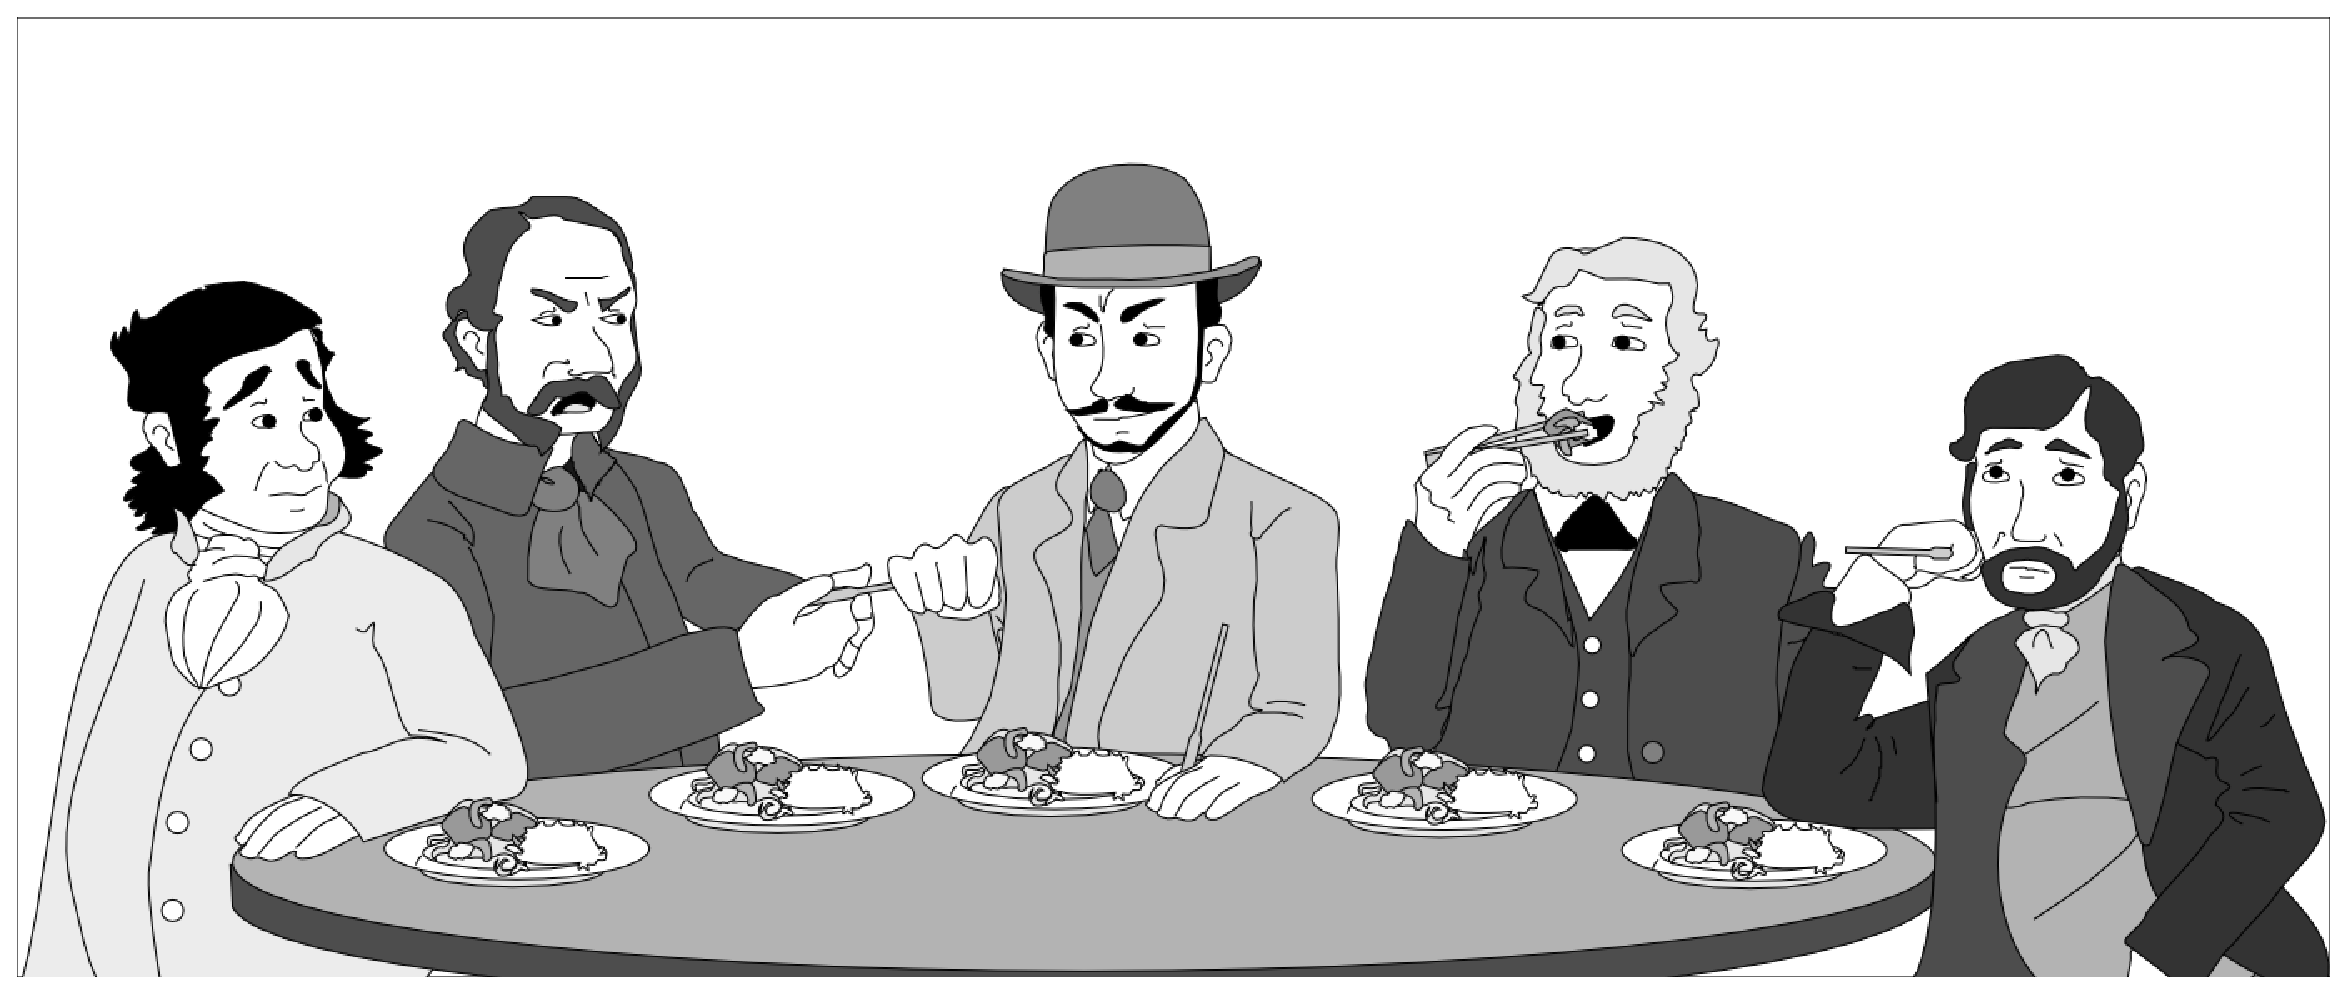
\includegraphics{cartoons/Dining-philosophers}}
\end{center}
\caption{Partial Starvation Is Also Bad}
\ContributedBy{Figure}{fig:cpu:Partial Starvation Is Also Bad}{Melissa Broussard}
\end{figure*}

목표는 스타베이션 (starvation: 기아) 을 막는 알고리즘을 만드는 것입니다.
스타베이션 시나리오 중 하나는 모든 철학자가 동시에 각자의 왼쪽 포크를 집어드는
것입니다.
그들은 스파게티를 다 먹기 전까지는 아무도 포크를 내려놓지 않을 것이고, 최소
한명은 식사를 끝내기 전까지는 두번째 포크를 들 수 없으므로, 그들 모두가
굶어죽게 됩니다.
최소 한명의 철학자는 먹게 해주는 것만으로는 문제 해결에 충분치 않음에
유의하시기 바랍니다.
Figure~\ref{fig:cpu:Partial Starvation Is Also Bad} 가 보이듯이, 일부 철학자의
스타베이션도 없어야 합니다.
\iffalse

The object is to construct an algorithm that, quite literally,
prevents starvation.
One starvation scenario would be if all of the philosophers picked up
their leftmost forks simultaneously.
Because none of them would put down their fork until after they ate,
and because none of them may pick up their second fork until at least
one has finished eating, they all starve.
Please note that it is not sufficient to allow at least one philosopher
to eat.
As Figure~\ref{fig:cpu:Partial Starvation Is Also Bad}
shows, starvation of even a few of the philosophers is to be avoided.
\fi

\begin{figure}[tb]
\begin{center}
\includegraphics[scale=.7]{SMPdesign/DiningPhilosopher5TB}
\end{center}
\caption{Dining Philosophers Problem, Textbook Solution}
\ContributedBy{Figure}{fig:SMPdesign:Dining Philosophers Problem, Textbook Solution}{Kornilios Kourtis}
\end{figure}

Dijkstra 의 해결책은 글로벌 세마포어를 사용하는 것으로, 무시해도 좋은 통신
딜레이를 가정하면 잘 동작하지만, 이 가정은 1980년대 후반이나 1990년대 초반
들어서는 타당하지 않게 되었습니다.\footnote{
	그 해결책이 나온지 40년이 넘게 지난 2012년의 관점에서 Dijkstra 를
	모욕하는 것은 너무도 쉽습니다.
	여전히 Dijkstra 를 모욕해야 겠다 생각한다면, 제가 드리고 싶은 말은,
	뭔가 출간하고, 40년 동안 기다린 후, \emph{당신의} 말들이 그 시간동안
	어떻게 검증되었는지 보시기 바랍니다.}
따라서, 최근의 해결책은 
Figure~\ref{fig:SMPdesign:Dining Philosophers Problem, Textbook Solution} 처럼
포크에 숫자를 매기는 것입니다.
각 철학자는 자신의 접시 옆의 것 중 가장 낮은 숫자의 포크를 먼저 들고, 이후에
가장 높은 숫자의 포크를 듭니다.
이 그림에서 가장 위쪽에 자리한 철학자는 따라서 왼쪽 포크를, 그 후 오른쪽 포크를
집어들게 되고, 그동안 다른 철학자들은 오른쪽 포크를 먼저 들게 됩니다.
두명의 철학자들은 포크~1 을 먼저 집어들으려 할 것이기 때문에, 그리고 두 철학자
중 한명만 성공할 것이기 때문에, 네명의 철학자들에게는 다섯개의 포크가 사용
가능할 것입니다.
이 네명 중 최소 한명은 두개의 포크를 집어드는데 성공함이 보장되고, 따라서
식사를 계속할 수 있습니다.
\iffalse

Dijkstra's solution used a global semaphore, which works fine assuming
negligible communications delays, an assumption that became invalid
in the late 1980s or early 1990s.\footnote{
	It is all too easy to denigrate Dijkstra from the viewpoint
	of the year 2012, more than 40 years after the fact.
	If you still feel the need to denigrate Dijkstra, my advice
	is to publish something, wait 40 years, and then see
	how \emph{your} words stood the test of time.}
Therefore, recent solutions number the forks as shown in
Figure~\ref{fig:SMPdesign:Dining Philosophers Problem, Textbook Solution}.
Each philosopher picks up the lowest-numbered fork next to his or her
plate, then picks up the highest-numbered fork.
The philosopher sitting in the uppermost position in the diagram thus
picks up the leftmost fork first, then the rightmost fork, while the
rest of the philosophers instead pick up their rightmost fork first.
Because two of the philosophers will attempt to pick up fork~1 first,
and because only one of those two philosophers will succeed,
there will be five forks available to four philosophers.
At least one of these four will be guaranteed to have two forks,
and thus be able to proceed eating.
\fi

이 일반적인 리소스에 숫자를 매기고 숫자 순서대로 획득하기 방법은 데드락 예방
기술에서 매우 많이 사용되고 있습니다.
하지만, 모두가 배고픈데 한번에 한명의 철학자만 식사를 하게 되는 경우를 초래하는
일련의 이벤트를 떠올리기는 쉽습니다:

\begin{enumerate}
\item	P2 가 포크~1 을 집어들고, P1 이 포크를 집어들지 못하게 합니다.
\item	P3 가 포크~2 를 집어듭니다.
\item	P4 가 포크~3 을 집어듭니다.
\item	P5 가 포크~4 를 집어듭니다.
\item	P5 가 포크~5 를 집어들고 식사를 합니다.
\item	P5 가 포크~4 와 5 를 내려놓습니다.
\item	P4 가 포크~4 를 집어들고 식사를 합니다.
\end{enumerate}
\iffalse

This general technique of numbering resources and acquiring them in
numerical order is heavily used as a deadlock-prevention technique.
However, it is easy to imagine a sequence of events that will result
in only one philosopher eating at a time even though all are hungry:

\begin{enumerate}
    \item P2 picks up fork~1, preventing P1 from taking a fork.
    \item P3 picks up fork~2.
    \item P4 picks up fork~3.
    \item P5 picks up fork~4.
    \item P5 picks up fork~5 and eats.
    \item P5 puts down forks~4 and 5.
    \item P4 picks up fork~4 and eats.
\end{enumerate}
\fi

즉, 다섯명의 철학자들이 모두 배고플 때에도, 두명의 철학자들이 동시에 식사를
해도 될만큼 충분한 양의 포크가 있음에도 한번에 한명의 철학자만 식사를 할 수
있는 경우가 존재합니다.

계속해서 읽기 전에 식사하는 철학자들 문제를 분할할 방법을 생각해 보시기
바랍니다.
\iffalse

In short, this algorithm can result in only one philosopher eating at
a given time, even when all five philosophers are hungry,
despite the fact that there are more than enough forks for two
philosophers to eat concurrently.

Please think about ways of partitioning the Dining Philosophers Problem
before reading further.
\fi
\cleardoublepage


\begin{figure}[tb]
\begin{center}
\includegraphics[scale=.7]{SMPdesign/DiningPhilosopher4part-b}
\end{center}
\caption{Dining Philosophers Problem, Partitioned}
\ContributedBy{Figure}{fig:SMPdesign:Dining Philosophers Problem, Partitioned}{Kornilios Kourtis}
\end{figure}

한가지 방법이 Figure~\ref{fig:SMPdesign:Dining Philosophers Problem,
Partitioned} 이 그려져 있는데, 이 방법을 좀 더 잘 그리기 위해 철학자들의 수를
다섯며에서 네명으로 바꿨습니다.
여기서 위쪽과 오른쪽의 철학자들은 한 짝의 포크를 공유하고, 아래쪽과 왼쪽의
철학자들은 다른 한짝의 포크를 공유합니다.
모든 철학자들이 동시에 배고파진다면, 최소 두명은 항상 동시적으로 식사를 할 수
있을 것입니다.
또한, 이 그림에서 보여지듯, 포크들은 동시에 집어들고 내려놓을 수 있도록
묶음으로 취급될 수 있어서 그 획득과 해제 알고리즘을 간단하게 만들어 줍니다.
\iffalse

One approach is shown in
Figure~\ref{fig:SMPdesign:Dining Philosophers Problem, Partitioned},
which includes four philosophers rather than five to better illustrate the
partition technique.
Here the upper and rightmost philosophers share a pair of forks,
while the lower and leftmost philosophers share another pair of forks.
If all philosophers are simultaneously hungry, at least two will
always be able to eat concurrently.
In addition, as shown in the figure, the forks can now be bundled
so that the pair are picked up and put down simultaneously, simplifying
the acquisition and release algorithms.
\fi

\QuickQuiz{}
	식사하는 철학자들 문제를 위한 더 나은 해결책은 없을까요?
	\iffalse

	Is there a better solution to the Dining
	Philosophers Problem?
	\fi
\QuickQuizAnswer{

\begin{figure}[tb]
\begin{center}
\includegraphics[scale=.7]{SMPdesign/DiningPhilosopher5PEM}
\end{center}
\caption{Dining Philosophers Problem, Fully Partitioned}
\QContributedBy{Figure}{fig:SMPdesign:Dining Philosophers Problem, Fully Partitioned}{Kornilios Kourtis}
\end{figure}

	그런 개선된 해결책이
	Figure~\ref{fig:SMPdesign:Dining Philosophers Problem, Fully Partitioned}
	에 보여져 있는데, 철학자들에게 추가로 다섯개의 포크를 주는 것입니다.
	이제 모든 다섯명의 철학자들이 동시에 식사를 할 수 있고, 따라서
	철학자들이 남을 기다려야 할 필요가 없습니다.
	또한, 이 방법은 질병 확산 제어를 엄청나게 개선시킵니다.

	이 해결책은 누군가에겐 사기처럼 보이겠지만, 그런 ``사기'' 가 많은
	동시성 문제에 좋은 해결책을 찾는 핵심입니다.
	\iffalse

	One such improved solution is shown in
	Figure~\ref{fig:SMPdesign:Dining Philosophers Problem, Fully Partitioned},
	where the philosophers are simply provided with an additional
	five forks.
	All five philosophers may now eat simultaneously, and there
	is never any need for philosophers to wait on one another.
	In addition, this approach offers greatly improved disease control.

	This solution might seem like cheating to some, but such
	``cheating'' is key to finding good solutions to many
	concurrency problems.
	\fi
} \QuickQuizEnd

이것은 두명씩으로 이루어진 철학자 그룹들 사이에 종속성이 없기 때문에, ``수평적
병렬성''~\cite{Inman85} 또는 ``데이터 병렬성'' 의 한가지 예입니다.
수평적으로 병렬적인 데이터 처리 시스템에서 데이터의 주어진 항목은 소프트웨어
컴포넌트들의 하나의 복제된 집합에서만 처리될 것입니다.
\iffalse

This is an example of ``horizontal parallelism''~\cite{Inman85}
or ``data parallelism'',
so named because there is no dependency among the pairs of philosophers.
In a horizontally parallel data-processing system, a given item of data
would be processed by only one of a replicated set of software
components.
\fi

\QuickQuiz{}
	그리고 어떤 관점에서 이 ``수평적 병렬성'' 은 ``수평적'' 이라 이야기 될
	수 있는 걸까요?
	\iffalse

	And in just what sense can this ``horizontal parallelism'' be
	said to be ``horizontal''?
	\fi
\QuickQuizAnswer{
	Inamn 은 프로토콜 스택에 대한 작업을 했는데, 이 프로토콜 스택은
	일반적으로는 어플리케이션을 꼭대기에 두고 하드웨어 연결을 바닥에 두는
	식으로 수직적으로 그림그려집니다.
	데이터는 이 스택의 위아래로 흐르게 됩니다.
	``수평적 병렬성'' 은 다른 네트워크 로부터의 패킷들을 병렬적으로
	처리하게 되는데, 반면 ``수직적 병렬성'' 은 각 패킷들에게 서로 다른
	프로토콜 처리 단계를 병렬적으로 줍니다.

	``수직적 병렬성'' 은 또한 ``파이프라이닝'' 이라고도 불립니다.
	\iffalse

	Inman was working with protocol stacks, which are normally
	depicted vertically, with the application on top and the
	hardware interconnect on the bottom.
	Data flows up and down this stack.
	``Horizontal parallelism'' processes packets from different network
	connections in parallel, while ``vertical parallelism''
	handles different protocol-processing steps for a given
	packet in parallel.

	``Vertical parallelism'' is also called ``pipelining''.
	\fi
} \QuickQuizEnd

\subsection{Double-Ended Queue}
\label{sec:SMPdesign:Double-Ended Queue}

Double-ended 큐는 원소가 양쪽의 끝 중 어디로든 삽입되고 삭제될 수 있는
자료구조입니다~\cite{Knuth73}.
동시에 양 끝으로 원소가 삽입 / 삭제될 수 있는 Double-ended 큐를 락 기반으로
구현하는 것은 어렵다고 알려져 있습니다~\cite{DanGrossman2007TMGCAnalogy}.
이 섹션은 세개의 일반적인 방법을 다음 섹션들에서 봄으로써 파티셔닝 디자인
전략이 어떻게 합리적으로 간단한 구현이 가능하게 하는지 알아봅니다.
\iffalse

A double-ended queue is a data structure containing a list of elements
that may be inserted or removed from either end~\cite{Knuth73}.
It has been claimed that a lock-based implementation permitting
concurrent operations on both ends of the double-ended queue is
difficult~\cite{DanGrossman2007TMGCAnalogy}.
This section shows how a partitioning design strategy can result
in a reasonably simple implementation, looking at three
general approaches in the following sections.
\fi

\subsubsection{Left- and Right-Hand Locks}
\label{sec:SMPdesign:Left- and Right-Hand Locks}

\begin{figure}[tb]
\begin{center}
\resizebox{3in}{!}{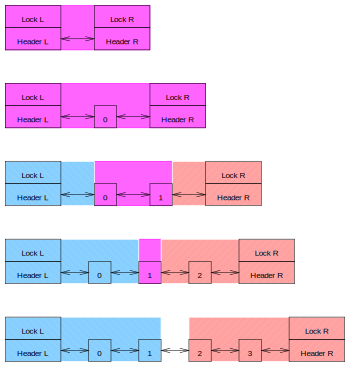
\includegraphics{SMPdesign/lockdeq}}
\end{center}
\caption{Double-Ended Queue With Left- and Right-Hand Locks}
\label{fig:SMPdesign:Double-Ended Queue With Left- and Right-Hand Locks}
\end{figure}

하나의 당연해 보이는 방법은 양방향 링크드 리스트를 왼쪽 인큐와 디큐를 위해 왼쪽
락을, 오른쪽 의 같은 작업들을 위해 오른쪽 락을 사용하는 것으로,
Figure~\ref{fig:SMPdesign:Double-Ended Queue With Left- and Right-Hand Locks}
에 그림으로 그려져 있습니다.
하지만, 이 방법의 문제는 두 락의 도메인들이 이 리스트에 원소가 네개보다 적을 때
겹치지 않아야 한다는 것입니다.
이 겹침은 어떤 원소의 삭제가 그 원소만이 아니라, 그것의 왼쪽 또는 오른쪽 이웃
원소에게도 영향을 끼치기 때문입니다.
이런 도메인들은 그림에 색으로 표시되었는데, 아래로 향하는 줄무늬의 파란색이
왼쪽 락의 도메인을, 위쪽 줄무늬의 붉은색이 오른쪽 락의 도메인을, 그리고 줄문의
없는 보라색은 겹치는 도메인들을 의미합니다.
이 방법으로 동작하는 알고리즘을 만드는 것도 가능하겠지만, 다섯개 미만의 특별한
케이스들이 있다는 사실은 커다란 문제인데, 특히나 리스트의 다른 끝에서의
동시적인 동작인 큐를 하나의 특별한 캐이스에서 다른 케이스로 언제든지 바꿀 수
있습니다.
다른 설계를 생각해 보는게 아무래도 낫습니다.
\iffalse

One seemingly straightforward approach would be to use a doubly
linked list with a left-hand lock
for left-hand-end enqueue and dequeue operations along with a right-hand
lock for right-hand-end operations, as shown in
Figure~\ref{fig:SMPdesign:Double-Ended Queue With Left- and Right-Hand Locks}.
However, the problem with this approach is that the two locks'
domains must overlap when there are fewer than four elements on the
list.
This overlap is due to the fact that removing any given element affects
not only that element, but also its left- and right-hand neighbors.
These domains are indicated by color in the figure, with blue
with downward stripes indicating
the domain of the left-hand lock, red with upward stripes
indicating the domain of the right-hand
lock, and purple (with no stripes) indicating overlapping domains.
Although it is possible to create an algorithm that works this way,
the fact that it has no fewer than five special cases should raise
a big red flag, especially given that concurrent activity at the other
end of the list can shift the queue from one special case to another
at any time.
It is far better to consider other designs.
\fi

\subsubsection{Compound Double-Ended Queue}
\label{sec:SMPdesign:Compound Double-Ended Queue}

\begin{figure}[tb]
\begin{center}
\resizebox{3in}{!}{\includegraphics{SMPdesign/lockdeqpair}}
\end{center}
\caption{Compound Double-Ended Queue}
\label{fig:SMPdesign:Compound Double-Ended Queue}
\end{figure}

락 도메인들이 겹치지 않게 하는 방법 한가지가
Figure~\ref{fig:SMPdesign:Compound Double-Ended Queue} 에 그려져 있습니다.
두개의 별도의 double-ended 큐를 직렬로 연결되며, 각각은 각자의 락으로
보호됩니다.
이는 원소들은 결국은 하나의 double-ended 큐에서 다른 것으로 옮겨가게 된다는
것을 의미하며, 이 경우 두 락을 모두 잡아야만 하게 됩니다.
데드락을 방지하기 위해 간단한 락 계층구조를 사용할 수 있는데, 예를 들면, 항상
오른쪽 락을 잡기 전에 왼쪽 락부터 잡는 것입니다.
이 방법은 조건 없이 왼쪽에 들어온 원소를 왼쪽의 큐에, 그리고 오른쪽으로 들어온
원소를 오른쪽 큐에 넣을 수 있기 때문에, 두개의 락을 하나의 double-ended 큐에
사용하는 것보다 훨씬 간단합니다.
빈 큐에서 원소를 꺼내려 할 때 좀 복잡한 문제가 생기는데, 이 경우에는 다음과
같은 작업이 필요합니다:
\iffalse

One way of forcing non-overlapping lock domains is shown in
Figure~\ref{fig:SMPdesign:Compound Double-Ended Queue}.
Two separate double-ended queues are run in tandem, each protected by
its own lock.
This means that elements must occasionally be shuttled from one of
the double-ended queues to the other, in which case both locks must
be held.
A simple lock hierarchy may be used to avoid deadlock, for example,
always acquiring the left-hand lock before acquiring the right-hand lock.
This will be much simpler than applying two locks to the same
double-ended queue, as we can unconditionally left-enqueue elements
to the left-hand queue and right-enqueue elements to the right-hand
queue.
The main complication arises when dequeuing from an empty queue, in
which case it is necessary to:
\fi

\begin{enumerate}
\item	오른쪽 락을 잡고 있다면, 그것을 해제부터 하고 왼쪽 락을 다시 잡는다.
\item	오른쪽 락을 잡는다.
\item	두 큐 사이의 원소들의 균형을 다시 잡는다.
\item	원소가 존재하면 요청받은대로 원소를 제거한다.
\item	두 락을 모두 놓는다.
\end{enumerate}
\iffalse

\begin{enumerate}
\item	If holding the right-hand lock, release it and acquire the
	left-hand lock.
\item	Acquire the right-hand lock.
\item	Rebalance the elements across the two queues.
\item	Remove the required element if there is one.
\item	Release both locks.
\end{enumerate}
\fi

\QuickQuiz{}
	이 compound double-ended 큐 구현에서, 비어있던 큐가 락을 놓고 다시 잡는
	과정 사이 더이상 비어있지 않게 된다면 어떻게 해야 할까요?
	\iffalse

	In this compound double-ended queue implementation, what should
	be done if the queue has become non-empty while releasing
	and reacquiring the lock?
	\fi
\QuickQuizAnswer{
	이 경우, 그냥 더이상 비어있지 않은 그 큐의 원소를 디큐하고, 락들을
	풀고, 리턴하면 그만입니다.
	\iffalse

	In this case, simply dequeue an item from the non-empty
	queue, release both locks, and return.
	\fi
} \QuickQuizEnd

그 결과로 만들어지는 코드 (\co{locktdeq.c}) 는 매우 직접적입니다.
앞서 언급한 다시 균형잡는 작업은 원소를 두 큐 사이에서 옮길 수도 있을 것이고,
이로 인해 시간을 소모할 수 있으므로 최적의 성능을 위해선 실제 워크로드에 따른,
휴리스틱이 필요할 것입니다.
어떤 경우엔 이게 최선의 방법이겠지만, 더 결정론적인 알고리즘을 시도해 보는 것도
재미있을 겁니다.
\iffalse

The resulting code (\co{locktdeq.c}) is quite straightforward.
The rebalancing operation might well shuttle a given element back
and forth between the two queues, wasting time and possibly requiring
workload-dependent heuristics to obtain optimal performance.
Although this might well be the best approach in some cases, it is
interesting to try for an algorithm with greater determinism.
\fi

\subsubsection{Hashed Double-Ended Queue}
\label{sec:SMPdesign:Hashed Double-Ended Queue}

One of the simplest and most effective ways to deterministically
partition a data structure is to hash it.
It is possible to trivially hash a double-ended queue by assigning
each element a sequence number based on its position in the list,
so that the first element left-enqueued into an empty queue is numbered
zero and the first element right-enqueued into an empty queue is numbered
one.
A series of elements left-enqueued into an otherwise-idle queue would
be assigned decreasing numbers (-1, -2, -3, ...), while a series of
elements right-enqueued into an otherwise-idle queue would be assigned
increasing numbers (2, 3, 4, ...).
A key point is that it is not necessary to actually represent a given
element's number, as this number will be implied by its position in
the queue.

\begin{figure}[tb]
\begin{center}
\resizebox{3in}{!}{\includegraphics{SMPdesign/lockdeqhash}}
\end{center}
\caption{Hashed Double-Ended Queue}
\label{fig:SMPdesign:Hashed Double-Ended Queue}
\end{figure}

Given this approach, we assign one lock to guard the left-hand index,
one to guard the right-hand index, and one lock for each hash chain.
Figure~\ref{fig:SMPdesign:Hashed Double-Ended Queue} shows the resulting
data structure given four hash chains.
Note that the lock domains do not overlap, and that deadlock is avoided
by acquiring the index locks before the chain locks, and by never
acquiring more than one lock of each type (index or chain) at a time.

\begin{figure}[tb]
\begin{center}
\resizebox{3in}{!}{
\includegraphics{SMPdesign/lockdeqhash1R}}
\end{center}
\caption{Hashed Double-Ended Queue After Insertions}
\label{fig:SMPdesign:Hashed Double-Ended Queue After Insertions}
\end{figure}

Each hash chain is itself a double-ended queue, and in this example,
each holds every fourth element.
The uppermost portion of
Figure~\ref{fig:SMPdesign:Hashed Double-Ended Queue After Insertions}
shows the state after a single element (``R1'') has been
right-enqueued, with the right-hand index having been incremented to
reference hash chain~2.
The middle portion of this same figure shows the state after
three more elements have been right-enqueued.
As you can see, the indexes are back to their initial states
(see Figure~\ref{fig:SMPdesign:Hashed Double-Ended Queue}), however,
each hash chain is now non-empty.
The lower portion of this figure shows the state after three additional
elements have been left-enqueued and an additional element has been
right-enqueued.

From the last state shown in
Figure~\ref{fig:SMPdesign:Hashed Double-Ended Queue After Insertions},
a left-dequeue operation would return element ``L-2'' and leave
the left-hand index referencing hash chain~2, which would then
contain only a single element (``R2'').
In this state, a left-enqueue running concurrently with a right-enqueue
would result in lock contention, but the probability of such contention
can be reduced to arbitrarily low levels by using a larger hash table.

\begin{figure}[tb]
\begin{center}
\resizebox{1.5in}{!}{
\includegraphics{SMPdesign/lockdeqhashlots}}
\end{center}
\caption{Hashed Double-Ended Queue With 12 Elements}
\label{fig:SMPdesign:Hashed Double-Ended Queue With 12 Elements}
\end{figure}

Figure~\ref{fig:SMPdesign:Hashed Double-Ended Queue With 12 Elements}
shows how 12 elements would be organized in a four-hash-bucket
parallel double-ended queue.
Each underlying single-lock double-ended queue holds a one-quarter
slice of the full parallel double-ended queue.

\begin{figure}[tbp]
{ \scriptsize
\begin{verbatim}
  1 struct pdeq {
  2   spinlock_t llock;
  3   int lidx;
  4   spinlock_t rlock;
  5   int ridx;
  6   struct deq bkt[DEQ_N_BKTS];
  7 };
\end{verbatim}
}
\caption{Lock-Based Parallel Double-Ended Queue Data Structure}
\label{fig:SMPdesign:Lock-Based Parallel Double-Ended Queue Data Structure}
\end{figure}

Figure~\ref{fig:SMPdesign:Lock-Based Parallel Double-Ended Queue Data Structure}
shows the corresponding C-language data structure, assuming an
existing \co{struct deq} that provides a trivially locked
double-ended-queue implementation.
This data structure contains the left-hand lock on line~2,
the left-hand index on line~3, the right-hand lock on line~4
(which is cache-aligned in the actual implementation),
the right-hand index on line~5, and, finally, the hashed array
of simple lock-based double-ended queues on line~6.
A high-performance implementation would of course use padding or special
alignment directives to avoid false sharing.

\begin{figure*}[bp]
{ \scriptsize
\begin{verbatim}
  1 struct cds_list_head *pdeq_pop_l(struct pdeq *d)
  2 {
  3   struct cds_list_head *e;
  4   int i;
  5 
  6   spin_lock(&d->llock);
  7   i = moveright(d->lidx);
  8   e = deq_pop_l(&d->bkt[i]);
  9   if (e != NULL)
 10     d->lidx = i;
 11   spin_unlock(&d->llock);
 12   return e;
 13 }
 14 
 15 struct cds_list_head *pdeq_pop_r(struct pdeq *d)
 16 {
 17   struct cds_list_head *e;
 18   int i;
 19 
 20   spin_lock(&d->rlock);
 21   i = moveleft(d->ridx);
 22   e = deq_pop_r(&d->bkt[i]);
 23   if (e != NULL)
 24     d->ridx = i;
 25   spin_unlock(&d->rlock);
 26   return e;
 27 }
 28 
 29 void pdeq_push_l(struct cds_list_head *e, struct pdeq *d)
 30 {
 31   int i;
 32 
 33   spin_lock(&d->llock);
 34   i = d->lidx;
 35   deq_push_l(e, &d->bkt[i]);
 36   d->lidx = moveleft(d->lidx);
 37   spin_unlock(&d->llock);
 38 }
 39 
 40 void pdeq_push_r(struct cds_list_head *e, struct pdeq *d)
 41 {
 42   int i;
 43 
 44   spin_lock(&d->rlock);
 45   i = d->ridx;
 46   deq_push_r(e, &d->bkt[i]);
 47   d->ridx = moveright(d->ridx);
 48   spin_unlock(&d->rlock);
 49 }
\end{verbatim}
}
\caption{Lock-Based Parallel Double-Ended Queue Implementation}
\label{fig:SMPdesign:Lock-Based Parallel Double-Ended Queue Implementation}
\end{figure*}

Figure~\ref{fig:SMPdesign:Lock-Based Parallel Double-Ended Queue Implementation}
(\co{lockhdeq.c}) 
shows the implementation of the enqueue and dequeue functions.\footnote{
	One could easily create a polymorphic implementation in any
	number of languages, but doing so is left as an exercise for
	the reader.}
Discussion will focus on the left-hand operations, as the right-hand
operations are trivially derived from them.

Lines~1-13 show \co{pdeq_pop_l()}, which left-dequeues and returns
an element if possible, returning \co{NULL} otherwise.
Line~6 acquires the left-hand spinlock, and line~7 computes the
index to be dequeued from.
Line~8 dequeues the element, and, if line~9 finds the result to be
non-\co{NULL}, line~10 records the new left-hand index.
Either way, line~11 releases the lock, and, finally, line~12 returns
the element if there was one, or \co{NULL} otherwise.

Lines~29-38 shows \co{pdeq_push_l()}, which left-enqueues the specified
element.
Line~33 acquires the left-hand lock, and line~34 picks up the left-hand
index.
Line~35 left-enqueues the specified element onto the double-ended queue
indexed by the left-hand index.
Line~36 then updates the left-hand index and line~37 releases the lock.

As noted earlier, the right-hand operations are completely analogous
to their left-handed counterparts, so their analysis is left as an
exercise for the reader.

\QuickQuiz{}
	Is the hashed double-ended queue a good solution?
	Why or why not?
\QuickQuizAnswer{
	The best way to answer this is to run \url{lockhdeq.c} on
	a number of different multiprocessor systems, and you are
	encouraged to do so in the strongest possible terms.
	One reason for concern is that each operation on this
	implementation must acquire not one but two locks.
	% Getting about 500 nanoseconds per element when used as
	% a queue on a 4.2GHz Power system.  This is roughly the same as
	% the version covered by a single lock.  Sequential (unlocked
	% variant is more than an order of magnitude faster!

	The first well-designed performance study will be cited.\footnote{
		The studies by Dalessandro
		et al.~\cite{LukeDalessandro:2011:ASPLOS:HybridNOrecSTM:deque}
		and Dice et al.~\cite{DavidDice:2010:SCA:HTM:deque} are
		good starting points.}
	Do not forget to compare to a sequential implementation!
} \QuickQuizEnd

\subsubsection{Compound Double-Ended Queue Revisited}
\label{sec:SMPdesign:Compound Double-Ended Queue Revisited}

This section revisits the compound double-ended queue, using a trivial
rebalancing scheme that moves all the elements from the non-empty
queue to the now-empty queue.

\QuickQuiz{}
	Move \emph{all} the elements to the queue that became empty?
	In what possible universe is this brain-dead solution in any
	way optimal???
\QuickQuizAnswer{
	It is optimal in the case where data flow switches direction only
	rarely.
	It would of course be an extremely poor choice if the double-ended
	queue was being emptied from both ends concurrently.
	This of course raises another question, namely, in what possible
	universe emptying from both ends concurrently would be a reasonable
	thing to do.
	Work-stealing queues are one possible answer to this question.
} \QuickQuizEnd

In contrast to the hashed implementation presented in
the previous section, the compound implementation will build on
a sequential implementation of a double-ended queue that uses
neither locks nor atomic operations.

\begin{figure*}[bp]
{ \scriptsize
\begin{verbatim}
  1 struct cds_list_head *pdeq_pop_l(struct pdeq *d)
  2 {
  3   struct cds_list_head *e;
  4 
  5   spin_lock(&d->llock);
  6   e = deq_pop_l(&d->ldeq);
  7   if (e == NULL) {
  8     spin_lock(&d->rlock);
  9     e = deq_pop_l(&d->rdeq);
 10     cds_list_splice(&d->rdeq.chain, &d->ldeq.chain);
 11     CDS_INIT_LIST_HEAD(&d->rdeq.chain);
 12     spin_unlock(&d->rlock);
 13   }
 14   spin_unlock(&d->llock);
 15   return e;
 16 }
 17 
 18 struct cds_list_head *pdeq_pop_r(struct pdeq *d)
 19 {
 20   struct cds_list_head *e;
 21 
 22   spin_lock(&d->rlock);
 23   e = deq_pop_r(&d->rdeq);
 24   if (e == NULL) {
 25     spin_unlock(&d->rlock);
 26     spin_lock(&d->llock);
 27     spin_lock(&d->rlock);
 28     e = deq_pop_r(&d->rdeq);
 29     if (e == NULL) {
 30       e = deq_pop_r(&d->ldeq);
 31       cds_list_splice(&d->ldeq.chain, &d->rdeq.chain);
 32       CDS_INIT_LIST_HEAD(&d->ldeq.chain);
 33     }
 34     spin_unlock(&d->llock);
 35   }
 36   spin_unlock(&d->rlock);
 37   return e;
 38 }
 39 
 40 void pdeq_push_l(struct cds_list_head *e, struct pdeq *d)
 41 {
 42   int i;
 43 
 44   spin_lock(&d->llock);
 45   deq_push_l(e, &d->ldeq);
 46   spin_unlock(&d->llock);
 47 }
 48 
 49 void pdeq_push_r(struct cds_list_head *e, struct pdeq *d)
 50 {
 51   int i;
 52 
 53   spin_lock(&d->rlock);
 54   deq_push_r(e, &d->rdeq);
 55   spin_unlock(&d->rlock);
 56 }
\end{verbatim}
}
\caption{Compound Parallel Double-Ended Queue Implementation}
\label{fig:SMPdesign:Compound Parallel Double-Ended Queue Implementation}
\end{figure*}

Figure~\ref{fig:SMPdesign:Compound Parallel Double-Ended Queue Implementation}
shows the implementation.
Unlike the hashed implementation, this compound implementation is
asymmetric, so that we must consider the \co{pdeq_pop_l()}
and \co{pdeq_pop_r()} implementations separately.

\QuickQuiz{}
	Why can't the compound parallel double-ended queue
	implementation be symmetric?
\QuickQuizAnswer{
	The need to avoid deadlock by imposing a lock hierarchy
	forces the asymmetry, just as it does in the fork-numbering
	solution to the Dining Philosophers Problem
	(see Section~\ref{sec:SMPdesign:Dining Philosophers Problem}).
} \QuickQuizEnd

The \co{pdeq_pop_l()} implementation is shown on lines~1-16
of the figure.
Line 5 acquires the left-hand lock, which line~14 releases.
Line~6 attempts to left-dequeue an element from the left-hand underlying
double-ended queue, and, if successful, skips lines~8-13 to simply
return this element.
Otherwise, line~8 acquires the right-hand lock, line~9
left-dequeues an element from the right-hand queue,
and line~10 moves any remaining elements on the right-hand
queue to the left-hand queue, line~11 initializes the right-hand queue,
and line~12 releases the right-hand lock.
The element, if any, that was dequeued on line~10 will be returned.

The \co{pdeq_pop_r()} implementation is shown on lines~18-38
of the figure.
As before, line~22 acquires the right-hand lock (and line~36
releases it), and line~23 attempts to right-dequeue an element
from the right-hand queue, and, if successful, skips lines~24-35
to simply return this element.
However, if line~24 determines that there was no element to dequeue,
line~25 releases the right-hand lock and lines~26-27 acquire both
locks in the proper order.
Line~28 then attempts to right-dequeue an element from the right-hand
list again, and if line~29 determines that this second attempt has
failed, line~30 right-dequeues an element from the left-hand queue
(if there is one available), line~31 moves any remaining elements
from the left-hand queue to the right-hand queue, and line~32
initializes the left-hand queue.
Either way, line~34 releases the left-hand lock.

\QuickQuiz{}
	Why is it necessary to retry the right-dequeue operation
	on line~28 of
	Figure~\ref{fig:SMPdesign:Compound Parallel Double-Ended Queue Implementation}?
\QuickQuizAnswer{
	This retry is necessary because some other thread might have
	enqueued an element between the time that this thread dropped
	\co{d->rlock} on line~25 and the time that it reacquired this
	same lock on line~27.
} \QuickQuizEnd

\QuickQuiz{}
	Surely the left-hand lock must \emph{sometimes} be available!!!
	So why is it necessary that line~25 of
	Figure~\ref{fig:SMPdesign:Compound Parallel Double-Ended Queue Implementation}
	unconditionally release the right-hand lock?
\QuickQuizAnswer{
	It would be possible to use \co{spin_trylock()} to attempt
	to acquire the left-hand lock when it was available.
	However, the failure case would still need to drop the
	right-hand lock and then re-acquire the two locks in order.
	Making this transformation (and determining whether or not
	it is worthwhile) is left as an exercise for the reader.
} \QuickQuizEnd

The \co{pdeq_push_l()} implementation is shown on lines~40-47 of
Figure~\ref{fig:SMPdesign:Compound Parallel Double-Ended Queue Implementation}.
Line~44 acquires the left-hand spinlock, line~45 left-enqueues the
element onto the left-hand queue, and finally line~46 releases
the lock.
The \co{pdeq_enqueue_r()} implementation (shown on lines~49-56)
is quite similar.

\subsubsection{Double-Ended Queue Discussion}
\label{sec:SMPdesign:Double-Ended Queue Discussion}

The compound implementation is somewhat more complex than the
hashed variant presented in
Section~\ref{sec:SMPdesign:Hashed Double-Ended Queue},
but is still reasonably simple.
Of course, a more intelligent rebalancing scheme could be arbitrarily
complex, but the simple scheme shown here has been shown to
perform well compared to software
alternatives~\cite{LukeDalessandro:2011:ASPLOS:HybridNOrecSTM:deque}
and even compared to algorithms using hardware
assist~\cite{DavidDice:2010:SCA:HTM:deque}.
Nevertheless, the best we can hope for from such a scheme
is 2x scalability, as at most two threads can be holding the
dequeue's locks concurrently.
This limitation also applies to algorithms based on non-blocking
synchronization, such as the compare-and-swap-based dequeue algorithm of
Michael~\cite{DBLP:conf/europar/Michael03}.\footnote{
	This paper is interesting in that it showed that special
	double-compare-and-swap (DCAS) instructions are not needed
	for lock-free implementations of double-ended queues.
	Instead, the common compare-and-swap (e.g., x86 cmpxchg)
	suffices.}

\QuickQuiz{}
	Why are there not one but two solutions to the double-ended queue
	problem?
\QuickQuizAnswer{
	There are actually at least three.
	The third, by Dominik Dingel, makes interesting use of
	reader-writer locking, and may be found in \co{lockrwdeq.c}.
} \QuickQuizEnd

In fact, as noted by Dice et al.~\cite{DavidDice:2010:SCA:HTM:deque},
an unsynchronized single-threaded double-ended queue significantly
outperforms any of the parallel implementations they studied.
Therefore, the key point is that there can be significant overhead enqueuing to
or dequeuing from a shared queue, regardless of implementation.
This should come as no surprise given the material in
Chapter~\ref{chp:Hardware and its Habits}, given the strict
FIFO nature of these queues.

Furthermore, these strict FIFO queues are strictly FIFO only with
respect to
\emph{linearization points}~\cite{Herlihy:1990:LCC:78969.78972}\footnote{
	In short, a linearization point is a single point within a given
	function where that function can be said to have taken effect.
	In this lock-based implementation, the linearization points
	can be said to be anywhere within the critical section that
	does the work.}
that are not visible to the caller, in fact, in these examples,
the linearization points are buried in the lock-based critical
sections.
These queues are not strictly FIFO with respect to (say) the times at which
the individual operations started~\cite{AndreasHaas2012FIFOisnt}.
This indicates that the strict FIFO property is not all that valuable
in concurrent programs, and in fact, Kirsch et al.~present less-strict
queues that provide improved performance and
scalability~\cite{ChristophMKirsch2012FIFOisntTR}.\footnote{
	Nir Shavit produced relaxed stacks for roughly the same
	reasons~\cite{Shavit:2011:DSM:1897852.1897873}.
	This situation leads some to believe that the linearization
	points are useful to theorists rather than developers, and
	leads others to wonder to what extent the designers of such
	data structures and algorithms were considering the needs
	of their users.}
All that said, if you are pushing all the data used by your concurrent
program through a single queue, you really need to rethink your
overall design.

\subsection{Partitioning Example Discussion}
\label{sec:SMPdesign:Partitioning Example Discussion}

The optimal solution to the dining philosophers problem given in
the answer to the Quick Quiz in
Section~\ref{sec:SMPdesign:Dining Philosophers Problem}
is an excellent example of ``horizontal parallelism'' or
``data parallelism''.
The synchronization overhead in this case is nearly (or even exactly)
zero.
In contrast, the double-ended
queue implementations are examples of ``vertical parallelism'' or
``pipelining'', given that data moves from one thread to another.
The tighter coordination required for pipelining in turn requires
larger units of work to obtain a given level of efficiency.

\QuickQuiz{}
	The tandem double-ended queue runs about twice as fast as
	the hashed double-ended queue, even when I increase the
	size of the hash table to an insanely large number.
	Why is that?
\QuickQuizAnswer{
	The hashed double-ended queue's locking design only permits
	one thread at a time at each end, and further requires
	two lock acquisitions for each operation.
	The tandem double-ended queue also permits one thread at a time
	at each end, and in the common case requires only one lock
	acquisition per operation.
	Therefore, the tandem double-ended queue should be expected to
	outperform the hashed double-ended queue.

	Can you created a double-ended queue that allows multiple
	concurrent operations at each end?
	If so, how?  If not, why not?
} \QuickQuizEnd

\QuickQuiz{}
	Is there a significantly better way of handling concurrency
	for double-ended queues?
\QuickQuizAnswer{
	One approach is to transform the problem to be solved
	so that multiple double-ended queues can be used in parallel,
	allowing the simpler single-lock double-ended queue to be used,
	and perhaps also replace each double-ended queue with a pair of
	conventional single-ended queues.
	Without such ``horizontal scaling'', the speedup is limited
	to 2.0.
	In contrast, horizontal-scaling designs can achieve very large
	speedups, and are especially attractive if there are multiple threads
	working either end of the queue, because in this
	multiple-thread case the dequeue
	simply cannot provide strong ordering guarantees.
	After all, the fact that a given thread removed an item first
	in no way implies that it will process that item
	first~\cite{AndreasHaas2012FIFOisnt}.
	And if there are no guarantees, we may as well obtain the
	performance benefits that come with refusing to provide these
	guarantees.
	% about twice as fast as hashed version on 4.2GHz Power.

	Regardless of whether or not the problem can be transformed
	to use multiple queues, it is worth asking whether work can
	be batched so that each enqueue and dequeue operation corresponds
	to larger units of work.
	This batching approach decreases contention on the queue data
	structures, which increases both performance and scalability,
	as will be seen in
	Section~\ref{sec:SMPdesign:Synchronization Granularity}.
	After all, if you must incur high synchronization overheads,
	be sure you are getting your money's worth.

	Other researchers are working on other ways to take advantage
	of limited ordering guarantees in
	queues~\cite{ChristophMKirsch2012FIFOisntTR}.
} \QuickQuizEnd

These two examples show just how powerful partitioning can be in
devising parallel algorithms.
Section~\ref{sec:SMPdesign:Locking Granularity and Performance}
looks briefly at a third example, matrix multiply.
However, all three of these examples beg for more and better design
criteria for parallel programs, a topic taken up in the next section.
